\documentclass[tikz,border=5pt]{standalone}
\usepackage{amsmath}
\usetikzlibrary{arrows.meta,positioning,calc}

\definecolor{obsfill}{HTML}{DDEBF7}
\definecolor{obsline}{HTML}{2F5597}
\definecolor{basefill}{HTML}{EFEFEF}
\definecolor{baseline}{HTML}{595959}
\definecolor{resfill}{HTML}{FBE5D6}
\definecolor{resline}{HTML}{C55A11}
\definecolor{predfill}{HTML}{E2F0D9}
\definecolor{predline}{HTML}{548235}
\definecolor{evalline}{HTML}{404040}
\definecolor{arrowline}{HTML}{333333}

\begin{document}
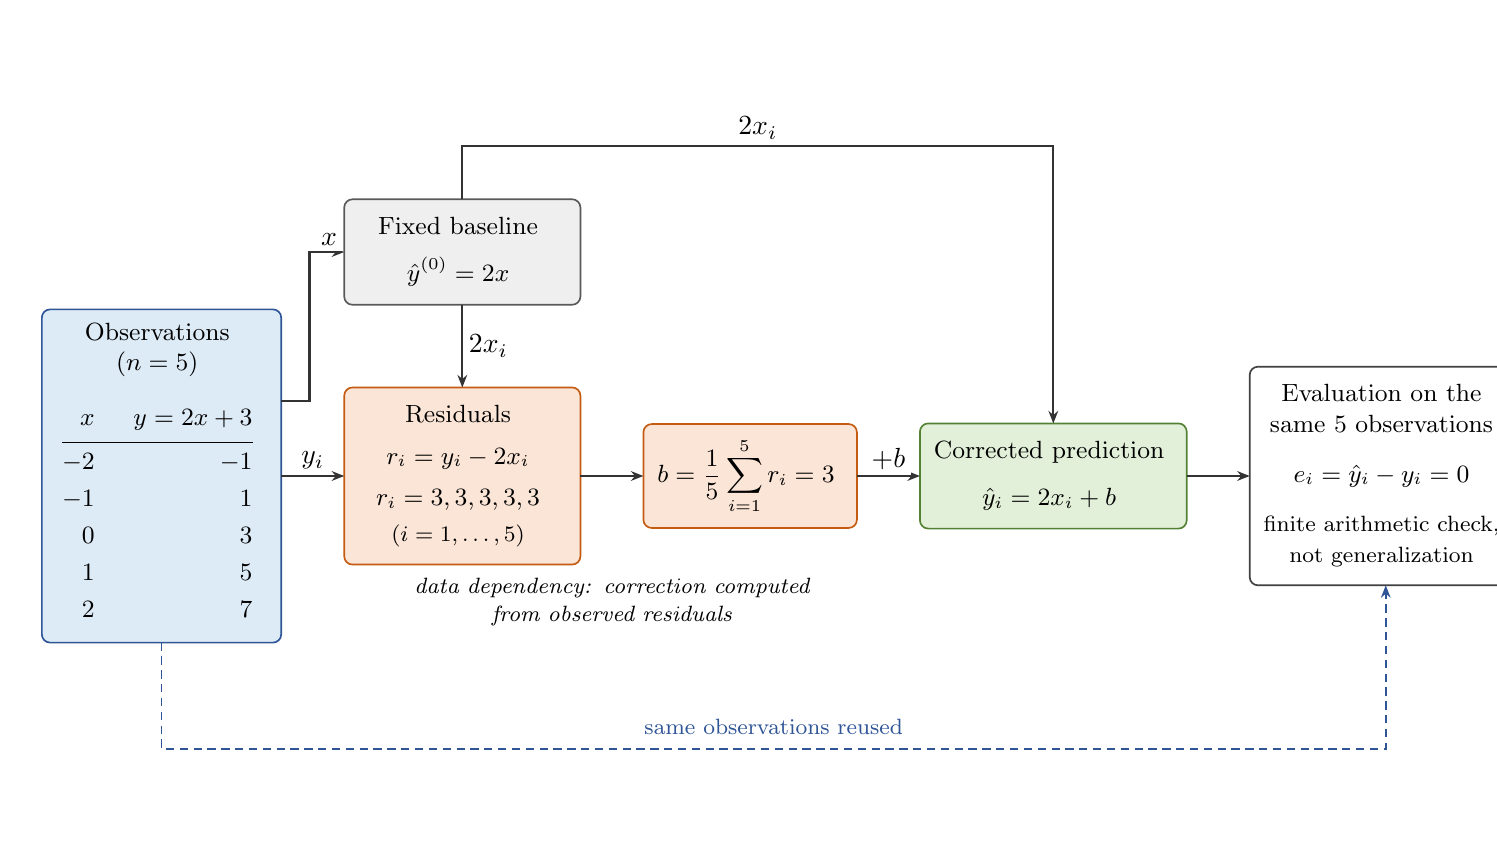
\begin{tikzpicture}[
    font=\fontsize{9}{11}\selectfont,
    block/.style={
        rectangle,
        rounded corners=3pt,
        line width=0.6pt,
        align=center,
        inner sep=5pt,
        outer sep=0pt
    },
    observation/.style={block,fill=obsfill,draw=obsline},
    baselineblock/.style={block,fill=basefill,draw=baseline},
    residualblock/.style={block,fill=resfill,draw=resline},
    prediction/.style={block,fill=predfill,draw=predline},
    evaluation/.style={block,fill=white,draw=evalline},
    computation/.style={
        draw=arrowline,
        line width=0.8pt,
        -{Stealth[length=4.5pt,width=3.5pt]}
    },
    reuse/.style={
        draw=obsline,
        line width=0.6pt,
        dash pattern=on 3pt off 2pt,
        -{Stealth[length=4.5pt,width=3.5pt]}
    },
    arrowlabel/.style={
        font=\fontsize{10}{12}\selectfont,
        fill=white,
        inner sep=2pt
    },
    annotation/.style={
        font=\fontsize{8}{10}\selectfont,
        align=center,
        inner sep=2pt
    }
]

% A landscape drawing area with a 16:9 aspect ratio.
\path[use as bounding box]
    (-1.70,-4.60) rectangle (16.60,5.69375);

% Stage 1: observations.
\node[observation,minimum width=3cm,minimum height=3.35cm]
    (observations) at (0,0) {%
    \begin{minipage}{2.58cm}
        \centering
        Observations ($n=5$)\\[7pt]
        \renewcommand{\arraystretch}{1.22}
        \setlength{\tabcolsep}{7pt}
        \begin{tabular}{@{}r r@{}}
            $x$ & $y=2x+3$\\[2pt]
            \hline
            $-2$ & $-1$\\
            $-1$ & $1$\\
            $0$  & $3$\\
            $1$  & $5$\\
            $2$  & $7$
        \end{tabular}
    \end{minipage}
};

% Stage 2: residuals and the fixed baseline, sharing one column.
\node[residualblock,
      minimum width=3cm,
      minimum height=1.65cm,
      right=0.8cm of observations]
    (residuals) {%
    \begin{tabular}{@{}c@{}}
        Residuals\\[4pt]
        $\displaystyle r_i=y_i-2x_i$\\[4pt]
        $r_i=3,3,3,3,3$\\[2pt]
        {\fontsize{8}{10}\selectfont $(i=1,\dots,5)$}
    \end{tabular}
};

\node[baselineblock,
      minimum width=3cm,
      minimum height=1.15cm,
      above=1.05cm of residuals]
    (fixedbaseline) {%
    \begin{tabular}{@{}c@{}}
        Fixed baseline\\[5pt]
        $\displaystyle \hat{y}^{(0)}=2x$
    \end{tabular}
};

% Stage 3: one scalar correction derived from the observed residuals.
\node[residualblock,
      minimum width=2.6cm,
      minimum height=1.15cm,
      right=0.8cm of residuals]
    (correction) {%
    $\displaystyle b=\frac{1}{5}\sum_{i=1}^{5}r_i=3$
};

% Stage 4: corrected prediction.
\node[prediction,
      minimum width=2.9cm,
      minimum height=1.30cm,
      right=0.8cm of correction]
    (corrected) {%
    \begin{tabular}{@{}c@{}}
        Corrected prediction\\[6pt]
        $\displaystyle \hat{y}_i=2x_i+b$
    \end{tabular}
};

% Stage 5: evaluation on the same observations.
\node[evaluation,
      minimum width=3.2cm,
      minimum height=2.15cm,
      right=0.8cm of corrected]
    (evaluate) {%
    \begin{tabular}{@{}c@{}}
        Evaluation on the\\
        same 5 observations\\[7pt]
        $\displaystyle e_i=\hat{y}_i-y_i=0$\\[7pt]
        {\fontsize{8}{10}\selectfont finite arithmetic check,}\\
        {\fontsize{8}{10}\selectfont not generalization}
    \end{tabular}
};

% Observation outputs use distinct anchors and separate routing corridors.
\coordinate (xout) at ($(observations.east)+(0,0.95)$);
\coordinate (xturn) at ($(xout)+(0.36,0)$);

\draw[computation]
    (xout) -- (xturn)
    |- node[arrowlabel,pos=0.78,above] {$x$}
    (fixedbaseline.west);

\draw[computation]
    (observations.east)
    -- node[arrowlabel,above] {$y_i$}
    (residuals.west);

% Baseline values enter the residual calculation vertically.
\draw[computation]
    (fixedbaseline.south)
    -- node[arrowlabel,right] {$2x_i$}
    (residuals.north);

% Residuals determine the correction.
\draw[computation]
    (residuals.east) -- (correction.west);

\coordinate (dependencycenter)
    at ($(residuals.east)!0.5!(correction.west)$);
\node[annotation,
      font=\fontsize{8}{10}\selectfont\itshape,
      text width=5.2cm,
      anchor=north]
    at ($(dependencycenter)+(0,-1.22)$)
    {data dependency: correction computed\\from observed residuals};

% The fixed baseline is also carried directly to the final predictor.
\coordinate (baselineroute)
    at ($(fixedbaseline.north)+(0,0.68)$);
\draw[computation]
    (fixedbaseline.north)
    -- (baselineroute)
    -- node[arrowlabel,above] {$2x_i$}
       (corrected.north |- baselineroute)
    -- (corrected.north);

\draw[computation]
    (correction.east)
    -- node[arrowlabel,above] {$+b$}
    (corrected.west);

\draw[computation]
    (corrected.east) -- (evaluate.west);

% Reuse is explicitly shown in a corridor below every block and annotation.
\coordinate (reuseleft) at ($(observations.south)+(0,-1.35)$);
\coordinate (reuseright) at (evaluate.south |- reuseleft);
\draw[reuse]
    (observations.south)
    -- (reuseleft)
    -- node[annotation,text=obsline,fill=white,above=3pt]
       {same observations reused}
       (reuseright)
    -- (evaluate.south);

\end{tikzpicture}
\end{document}